\documentclass{article}
\usepackage[utf8]{inputenc}
\usepackage[a4paper,top=1in,bottom=1in,left=1in,right=1in,marginparwidth=1.75cm]{geometry}
\usepackage{amssymb,amsmath,amsthm,gensymb,enumitem,textcomp,mathtools}

\newenvironment{packed_enum}{
	\begin{enumerate}
		\setlength{\itemsep}{1pt}
		\setlength{\parskip}{0pt}
		\setlength{\parsep}{0pt}
	}{\end{enumerate}}

\newcommand{\methane}{$\mathrm{CH_4}$}
\newcommand{\popt}{\mathbf{\Pi_{\mathrm{opt}}}}
\newcommand{\g}{\Gamma}
\newcommand{\gstar}{\Gamma^{\star}}

% General inversion terms
\newcommand{\const}{\mathbf{c}}
\newcommand{\x}{\mathbf{x}}
\newcommand{\xa}{\mathbf{x}_{\mathrm{A}}}
\newcommand{\y}{\mathbf{y}}
\newcommand{\K}{\mathbf{K}}
\newcommand{\so}{\mathbf{S}_{\mathrm{O}}}
\newcommand{\sa}{\mathbf{S}_{\mathrm{A}}}

% Posterior solutions
\newcommand{\xpost}{\mathbf{\hat{x}}}
\newcommand{\spost}{\mathbf{\hat{S}}}
\newcommand{\A}{\mathbf{A}}

% Reduced rank solutions
\newcommand{\xpostpi}{\mathbf{\hat{x}}_{\popt}}
\newcommand{\spostpi}{\mathbf{\hat{S}}_{\popt}}
\newcommand{\Api}{\mathbf{A}_{\popt}}
\newcommand{\dof}[1]{#1_\mathrm{DOF}}
\newcommand{\pidof}{\dof{\mathbf{\Pi}}}
\newcommand{\xpostdof}{\mathbf{\hat{x}}_{\pidof}}
\newcommand{\spostdof}{\mathbf{\hat{S}}_{\pidof}}
\newcommand{\Adof}{\mathbf{A}_{\pidof}}

\title{Reducing Jacobian Computational Cost}
\author{Hannah Nesser}
\date{October 2018}

\begin{document}
\maketitle
\section{Introduction}
%Atmospheric methane levels have increased 2.5 times since the preindustrial era, from 720 ppb to over 1860 ppb in September 2018 (cite NOAA). This increase has a significant climate effect: methane is the second largest contributor to radiative forcing after carbon dioxide (cite IPCC). Because methane has a shorter lifetime than carbon dioxide, reducing its emissions will decrease short-term contributions to climate change (cite something). Of the IPCC emission reduction pathways that limit global warming to 1$\degree$ C with no or limited overshoot, all involve deep reductions in methane emisisons (insert citation).\\
%\\
%Methane is the second largest contributor to radiative forcing after carbon dioxide (cite IPCC). 
All emission reduction pathways that limit global warming to 1$\degree$ C with no or limited overshoot involve deep reductions in methane emisisons (insert IPCC citation). Global methane emissions of 550 $\mathrm{Tg \hspace{1mm} a^{-1}}$ are well constrained by inference from mass balance with the global methane sink (Jacob 2016) and the biogenic and anthropogenic sources, including wetlands, livestock, oil and gas systems, landfills, coal mines, and rice paddies, are well known. However, the spatial and temporal contributions of different sources and regions are highly uncertain (cite Kirschke 2013, etc). Satellite observations of total methane columns can constrain bottom-up estimates of methane emissions within the framework of a Bayesian inversion. As satellite technology evolves, inversions are able to constrain methane emissions at increasingly high resolutions. However, as the resolution of an analytic inversion increases, the computational cost increases significantly. Here, we develop a method to decrease the computational cost of analytic Bayesian inversions by applying reduced rank methods to the construction of the Jacobian.\\
\\
Bayesian inversions calculate the spatially- and temporally-resolved emissions that optimize both prior and observational errors, given a forward model for atmospheric chemistry and transport. When the forward model is linear, there is a closed-form solution for the posterior emissions estimate and its error. The information content of the posterior solution is given by the averaging kernel $\A$ and, in particular, by the trace of $\A$, which gives the Degrees Of Freedom for Signal (DOFS), the number of pieces of information the inversion can constrain.\\
\\
The computational cost of an analytic inversion is limited by the dimension of the emission (state) vector, which defines the cost of (1) generating the Jacobian $\K$, which requires $n+1$ forward model runs, and of (2) solving the analytic expression for the posterior error covariance, which requires the inversion of a non-sparse $n \times n$ matrix. Analytic Bayesian inversions of GOSAT observations frequently constrained emissions on a $4\degree \times 5\degree$ grid, generating a posterior estimate for $n \approx 1,000$ continental grid cells (i.e. Turner, Maasakkers, Zeng, etc.). TROPOMI aboard the Sentinel-5 Precursor, a satellite launched by the European Space Agency in October 2017, will return methane observations at much higher resolution and density than GOSAT: GOSAT provided approximately 2 million methane column measurements from 2009 to 2015 [cite Maassakkers]; TROPOMI could return this quantity of data in four days [cite Hu]. With this increase in data density, Bayesian inversions will be able to constrain emissions on a much finer grid, increasing the dimension of the state vector from $n \approx 1,000$ to $n \approx 4,000$ or $n \approx 16,000$.\\
\\
Past work has focused on decreasing the computational cost of calculating the poterior error covariance. [Insert material on variational inference, ensemble Kalman filters, etc.] Bocquet et al. (2011) defined a method to find a reduced-dimension state vector that maximized the DOFS of the system; however, this method required the construction of many aggregated grids, reducing the computational benefit of the dimension reduction. Turner et al. (2015) also reduced the dimension of the state vector, but constrained emissions on a set of Gaussian radial basis functions rather than an aggregated grid. However, this set of Gaussians did not guarantee optimality. Spantini et al. (2015) defined low-rank approximations that maximized the DOFS of the low-rank system by constructing an optimal, low-rank projection. Bousserez et al. (2018) built upon the framework developed by Bocquet et al. and by Spantini et al. and defined additional, improved approximations and closed-form expressions for the error of the reduced-rank solution relative to the full-rank solution. However, none of these methods addressed the computational cost of constructing the Jacobian $\K$.\\
\\
In what follows, I describe a method to reduce the computational cost of constructing the Jacobian $\K$ that builds upon the reduced-rank framework developed by Bousserez et al. (2018). In section \ref{theory}, I discuss the theoretical basis of this method. In section \ref{demo}, I present the results from the application of this method to a high-resolution inversion of GOSAT observations over North America.

\section{Reduced-Rank Bayesian Inversions and Jacobians}{\label{theory}}
% Explain general idea of reduced rank
Bayesian inversions calculate the spatially- and temporally-resolved emissions that optimize both prior and observational errors, given a forward model for atmospheric chemistry and transport. If the forward model is linear, then the Jacobian $\K$ describes the linear map between the emissions space $E$ with dimension $n$ and the observations space $F$ with dimension $m$: $\K : E \rightarrow F$. In other words, for $\x \in E$ and $\y \in F$, $\y = \K\x + \mathbf{c}$. When using satellite observations, it is often the case that $m \gg n$, producing a problem that is, in the classical sense, overconstrained. However, the number of pieces of information $n_{DOF}$ that can be constrained by an inversion is often less than the number of state vector elements: $n_{DOF} \ll n$; the problem is in fact underconstrained. In the underconstrained linear system, the rank $k$ of the Jacobian $\K$ is less than the upper bound $n$. Reduced rank inversion schemes, as introduced by Spantini et al. (2015) and elaborated on by Bousserez et al. (2018), solve analytic Bayesian inversions in a reduced rank space, decreasing the computational cost of inverting a non-sparse $n \times n$ matrix. However, these approaches do not address the computational cost of constructing the Jacobian $\K$.\\
\\
In what follows, we describe the standard approach to Bayesian inversions (Section \ref{full_dim_invs}) and the reduced rank approach developed by Spantini et al. (2015) and Bousserez et al. (2018) (Section \ref{red_rank_invs}). We then introduce the reduced rank approach to Jacobian construction (Section \ref{red_rank_k}) and develop error characterization for the approach (Section \ref{error_char}).

\subsection{Bayesian Inversions and Jacobians}{\label{full_dim_invs}}
A Bayesian inversion assumes that prior and observational errors are Gaussian and minimizes a cost function $\mathit{J}$:
\begin{align}
	\mathcal{J}(\x) &= \frac{1}{2}(\y - K(\x))^\mathrm{T}\so^{-1}(\y - K(\x)) + \frac{1}{2}(\x - \xa)^\mathrm{T}\sa^{-1}(\x - \xa)
\end{align}
where $\x$ is the state vector, $\xa$ is the vector of prior emissions, $\y$ is the vector of observations, $K$ is the forward model, and $\sa$ and $\so$ are the prior and observational error covariance matrices, respectively. When the forward model is linear, $K(\x) = \K\x + \const$, and there is an analytic solution that minimizes $\mathcal{J}(\x)$, giving the posterior $\xpost$. There is also an analytic solution for the posterior error $\spost$ and for the information content of the system, given by the averaging kernel $\A$. The Bayesian linear problem may be written as $\{\mathcal{B} : \y \vert \x \sim \mathcal{N}(\K\x, \so);\ \x \sim \mathcal{N}(\mathbf{0}, \sa);\ \x \in E,\ \y \in F\}$. To simplify notation, we use the formalism of Bousserez et al. (2018): $\mathcal{B} \equiv (E, F, \K, \sa, \so)$.\\
\\
The computational cost of an analytic inversion is dominated by the time it takes to (1) define the linear relationship between the observations and emissions and (2) calculate the posterior error covariance. In both cases, the computational cost is limited by the dimension $n$ of the state vector $\x$. In the former case, an $n \times n$ matrix must be inverted to calculate the posterior error covariance. In the latter case, the Jacobian is constructed column-wise by running a $n$ perturbation experiments in the forward model. In a given experiment, one state vector element is perturbed, and the model output is compared to a base run. This gives $d\y/d\x_i$, a single column of the Jacobian, where $i = {1, ... , n}$. Using the adjoint instead of the Jacobian may decrease the computational cost of the first inversion, but the cost increases with subsequent inversions (i.e. sensitivity tests). Once the Jacobian is built, it may be used for a series of inversions, including sensitivity tests. It is therefore the preferred method.\\
\\
(Insert transition)

\subsection{Reduced-Rank Bayesian Inversions}{\label{red_rank_invs}
A reduced-rank inversion solves the inverse problem in a subspace of the original state space. Bousserez et al. (2018) defined a rank-k projection operator $\Pi$ that translates the Bayesian inversion to this subspace. Like any rank-k linear operator, $\Pi$ may be written as the product of two rank-k matrices, one which is the left inverse of the other:
\begin{align}
	\Pi &= \gstar\g
\end{align}
where $\gstar$ has dimension $n \times k$ and $\g$ has dimension $k \times n$. The projection may therefore be understood as a sequence of two operations: the first, $\g$, reduces the dimension of the state vector from $n$ to $k$, while the second, $\gstar$, increases the dimension from $k$ to $n$. I will refer to $\g$ as the reduction operator and $\gstar$ as the prolongation operator, keeping with the formalism of Bousserez et al. (2018).\\
\begin{figure}[h]
	\begin{center}
		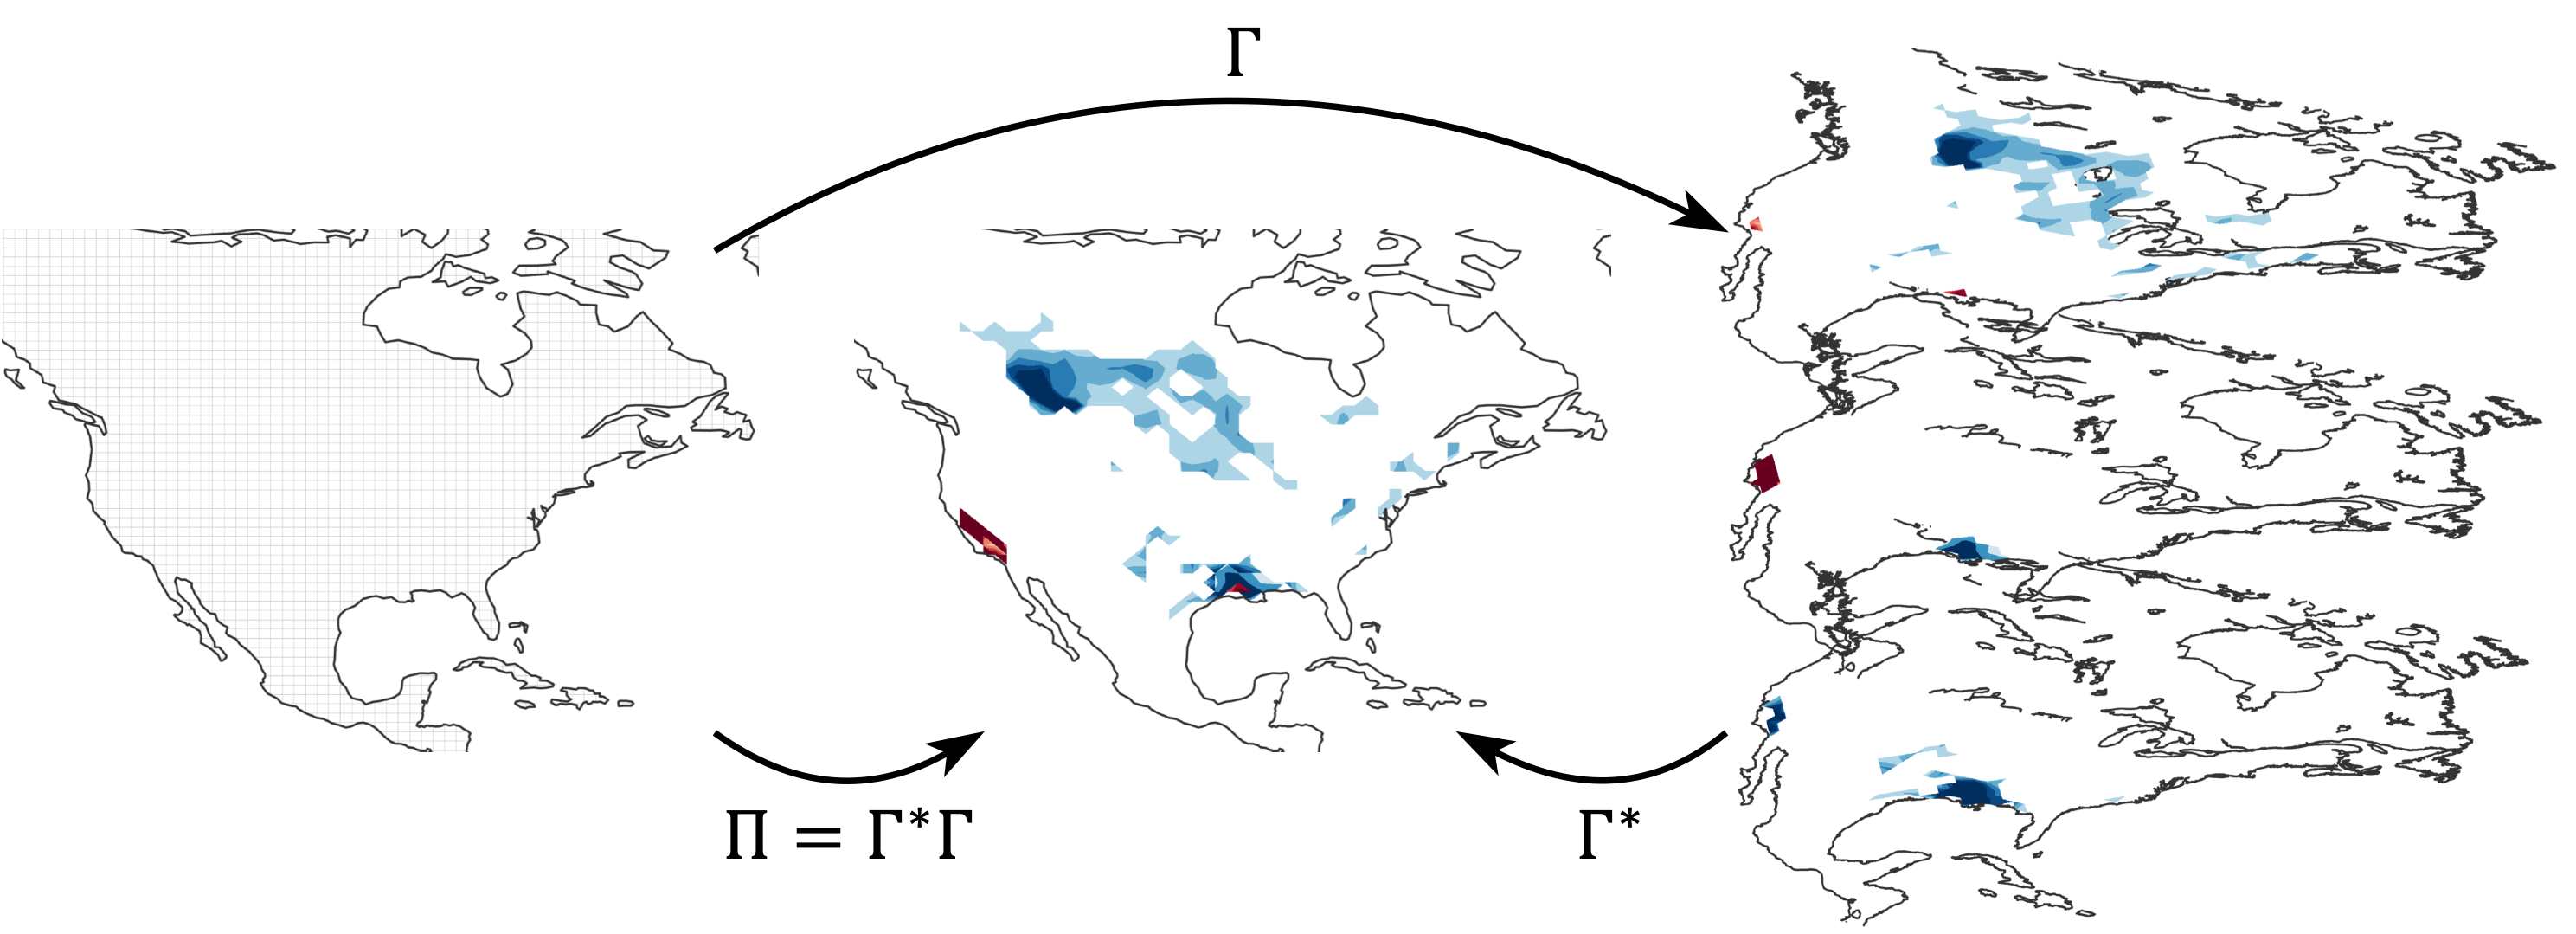
\includegraphics[width=6in]{dim_rank_scheme.png}
		\caption{\textit{Note: this chart is adapted from Bocquet et al. (2009). I will modify the chart to more accurately reflect our scheme (i.e. representing non-discrete elements of the subspace w) at a later date.}}
		\label{space_flow_chart}
	\end{center}
\end{figure}\\
Figure \ref{space_flow_chart} shows the relationship between the  original emission-observation space, the projected subspace, and the reduced dimension subspace. The original space of the problem is depicted by the leftmost panel. The rank $k$ projection $\mathbf{\Pi}$ transforms the original space to a rank $k$ subspace, depicted by the center panel. The reduction operator $\g$ transforms the reduced rank subspace to a reduced dimension subspace, depicted by the right panel. The optimal prolongation operator $\gstar$ returns the reduced dimension space to the reduced rank subspace. However, there is no operator defining a return to the orignal space. Qualitatively, reducing the rank of the original space involves a loss of information that cannot be restored. Quantiatively, the projector $\mathbf{\Pi}$ is of dimension $n \times n$ but rank $k$, meaning that it is non-invertible and the transformation cannot be precisely reversed.\\
\\
The projected Bayesian problem corresponds to the center panel of Figure \ref{space_flow_chart}. Its posterior solution correspond to the posterior solution in the original space projected to the reduced rank subspace. Specifically,
\begin{align}
	\xpostpi &= \Pi \xpost\\
	\spostpi &= \Pi \spost \Pi^{\mathrm{T}}\\
	\Api &= \Pi \A \Pi	
\end{align}\\
The rank $k$ projection $\mathbf{\Pi}$ necessarily discards information. However, a projection can be found that optimizes some criteria, such as minimal information content loss. Of particular interest is the minimization of the representativeness error, which is the error introduced if the subspace of the observations is not fully included in the range of the projector; it is the difference between the full-rank observational error and the observational error of the reduced-rank system. Bousserez et al. (2018) describe a general form of a projection that minimizes representativeness error; in particular, they show that for any reduction operator $\g$ there exists a prolongation operator $\gstar$ that minimizes representativeness error:
\begin{align}
	\gstar_{opt} = \sa\g^{\mathrm{T}}(\g\sa\g^{\mathrm{T}})^{-1}
\end{align}
Within this class of projections, additional optimality criteria, such as maximizing the DOFS or minimizing the posterior variance, can be introduced. Bousserez et al. (2018) find that it is possible to create representativeness-error minimizing projection that also maximizes the DOFS of the reduced-rank inversion. This projection is given by:
\begin{align}\label{dof_projection}
	\dof{\mathbf{\Pi}} &= \sa^{1/2}\mathbf{W}_k\mathbf{W}_k^{\mathrm{T}}\sa^{-1/2}
\end{align}
$\mathbf{W}_k$ is the matrix whose columns are the first k eigenvectors of the prior-error-weighted averaging kernel $\dof{\mathbf{Q}} \equiv \sa^{-1/2}\A\sa^{1/2}$ with eigendecomposition $\dof{\mathbf{Q}} = \mathbf{W}^{\mathrm{T}} \mathbf{\Sigma} \mathbf{W}$, where $\mathbf{W}$ is the matrix whose columns are the eigenvectors of $\dof{\mathbf{Q}}$ and $\mathbf{\Sigma}$ is a diagonal matrix whose elements are the eigenvalues of $\mathbf{\Sigma}$. However, this solution requires the inversion of a non-sparse $n \times n$ matrix, negating any benefit to the computational cost. Bousserez et al. (2018) find that the eigenpairs of $\dof{\mathbf{Q}}$ are linearly related to those of another matrix, the prior-preconditioned Hessian $\mathbf{H}_{\mathrm{p}} \equiv \sa^{1/2}\K^{\mathrm{T}}\so^{-1}\K\sa^{1/2}$ with eigendecomposition $\mathbf{H}_{\mathrm{p}} = \mathbf{V}^{\mathrm{T}} \mathbf{\Lambda} \mathbf{V}$. The eigenvectors and eigenvalues of the prior-preconditioned Hessian are related to those of $\dof{\mathbf{Q}}$ by the following linear relationships:
\begin{align}
\mathbf{W} &= \mathbf{V}\\
\mathbf{\Sigma} &= \mathbf{\Lambda}(\mathbf{I} + \mathbf{\Lambda})^{-1}
\end{align}
Given the eigendecomposition of the prior-preconditioned Hessian, the optimal reduction and prolongation operators are:
\begin{align}
	\label{reduction_op}\g &= \mathbf{V}_k^{\mathrm{T}}\sa^{-1/2}\\
	\label{prolongation_op}\gstar &= \sa^{1/2}\mathbf{V}_k
\end{align}
(Personal note: This is a correction of the result presented by Bousserez et al. (2018).)\\
\\
It is then possible to write the posterior solution of a DOFS maximizing rank k projection:
\begin{align}
	\xpostdof &= \sa^{1/2}\left( \sum_{i = 1}^{k} \lambda_i^{1/2}(1+\lambda_i)^{-1}\mathbf{v}_i\mathbf{w}_i^{\mathrm{T}}  \right)\so^{-1/2}(\y - (\K\x + \const))\\
	\spostdof &= \sa^{1/2}\left( \sum_{i=1}^{k} (1+\lambda_i)^{-1}\mathbf{v}_i\mathbf{v}_i^\mathrm{T} \right)\sa^{1/2}\\
	\Adof &= \sa^{1/2} \left( \sum_{i=1}^{k} \lambda_i(1+\lambda_i)^{-1}\mathbf{v}_i\mathbf{v}_i^\mathrm{T} \right)\sa^{-1/2}
\end{align}
If all eigenvectors and eigenvalues of the prior-preconditioned Hessian are explicitly calculated (and not approximated using random SVD), the posterior mean may be written:
\begin{align}
	\xpostdof &= \spostdof \K^{\mathrm{T}} \so^{-1}(\y - (\K\x + \const))\\
\end{align}
These are solutions to the projected problem $\mathcal{B}_{\pidof} \equiv (E_{\pidof},F,\K,\mathbf{S}_{\mathrm{A}_{\pidof}}, \mathbf{S}_{\mathrm{O}_{\pidof}})$. It is also possible to define the problem $\mathcal{B}_{\K_{\pidof}} \equiv (E,F,\K\pidof,\sa, \mathbf{S}_{\mathrm{O}_{\pidof}})$, which corresponds to the initial inverse problem with a projected forward model. The posterior solutions of that problem are:
\begin{align}
	\xpost_{\K_{\pidof}} &= \xpostdof\\
	\spost_{\K_{\pidof}} &= \spostdof + \sa^{1/2} \left( \sum_{i = k+1}^{n} \mathbf{v}_i \mathbf{v}_i^\mathrm{T} \right) \sa^{1/2}\\
	&= \sa -  \sa^{1/2}\left( \sum_{i=1}^{k} \lambda_i(1+\lambda_i)^{-1}\mathbf{v}_i\mathbf{v}_i^\mathrm{T} \right)\sa^{1/2}\\
	\A_{\K_{\pidof}} &= \Adof
\end{align}
The posterior error covariance associated with the projected forward model is similar to that of the maximum DOFS projection, but corresponds to "a forward model for which the modes are filtered by the projection $\pidof$" (Bousserez et al. (2018)). (Edit. Also note which set of solutions is preferable.)\\
\\
(Insert transition)
%It is worth nothing that both sets of solutions are in terms of the full-rank, non-projected Jacobian and error covariance matrices. However, if the computational cost of constructing the Jacobian is reduced by generating a reduced-rank Jacobian $\K_{\pidof} = \K \pidof$, these results must be expressed in terms of the reduced-rank Jacobian. I present those results in what follows.

%\subsubsection{Projected Forward Model Solutions}
\subsection{Reduced-Rank Jacobian Construction}{\label{red_rank_k}
In a standard inversion, the Jacobian is constructed column-wise by conducting $n+1$ model runs, where in model run $i+1$, the $i$th grid cell is perturbed. In a reduced-rank inversion, the elements of the reduced-dimension space $\omega$ with dimension $k \ll n$ may be perturbed instead. However, defining the optimal projection and its reduction and prolongation operators requires prior knowledge of the Jacobian (insert equation reference). Therefore, it is necessary to iteratively update the reduced-rank Jacobian estimate. In what follows, we assume $\mathbf{\Pi} = \pidof$.\\
\\
The general iteration scheme is as follows: \textit{Note: here I enumerate the general approach, considering all possible iteration routes. I will go into more detail on each of the routes, and on their sticking points, later.)}
\begin{packed_enum}%[label=(\roman*)]
	\item Initialize the Jacobian $\K_0$. 
	\item Solve for the associated rank-$k$ optimal projection $\mathbf{\Pi}_0 = \gstar_0\g_0$.
	\item Perturb some $k$ elements (either eigenvectors or grid cells) and calculate the associated Jacobian. The Jacobian may be in (a) the projected subspace (i.e. the subspace defined by $\mathbf{\Pi}$), (b) the reduced dimension space (i.e. $\omega$, the subspace defined by $\g$), or (c) the original space.
	%	\item Perturb the projected prior $\x_{\mathrm{A}\Pi} = \mathbf{\Pi}_0 \xa$ $k$ times. This gives $\K_{\omega_{0}}$, from which $\K_{\Pi_0}$ can be calculated as $\K_{\Pi_0} = \K_{\omega_{0}}\g$. Then estimate the non-projected, updated Jacobian: $\K_1 = (\mathbf{Id}_n - \mathbf{\Pi}_0)\K_0 + \K_{\Pi_0}$.
	\item Return to item 2 and iterate until convergence.
	\item Solve the inversion. If the final Jacobian is in the projected subspace or the reduced dimension space, the solution will be within that space.\\
\end{packed_enum}
The Jacobian may be initialized by, for instance, generating a Jacobian at coarser resolution and regridding. Changes in modeled observations at coarse resolution may be allocated to higher resolution grid cells according to the fraction of emissions the smaller grid cell is responsible for relative to the larger grid cell, with the fraction given by the prior estimate. For a coarse grid cell with emissions $x$ with higher resolution consituents $x_1,\ x_2,\ x_3,$ and $x_4$ and an observation vector $\y$ that we wish to decompose into its higher resolution constituents $\y_1,\ \y_2,\ \y_3,$ and $\y_4$:
\begin{align*}
\frac{\Delta \y}{\Delta x} &= \frac{\Delta  \y_1 + \Delta \y_2 + \Delta \y_3 + \Delta \y_4}{\Delta x_1 + \Delta x_2 + \Delta x_3 + \Delta x_4}\\
\Delta  \y_1 + \Delta \y_2 + \Delta \y_3 + \Delta \y_4 &= f_1\Delta \y + f_2 \Delta \y + f_3 \Delta \y + f_4 \Delta \y
\end{align*}
We then estimate $\Delta \y_i \approx f_i \Delta \y$ for $i \in \{1,\ 2,\ 3,\ 4\}$, where $f_i = \Delta x_i / \Delta x$, the fraction of the coarse grid cell emissions attributable to the smaller cell. The approximate changes in observations at fine resolution are then used to calculate an initial estimate of the Jacobian $\K_0$.\\
\\
However, building a coarse resolution Jacobian reduces the computational benefit of the reduced rank approach since it requires at maximum $n/4$ and down to $n/8$ or $n/16$ model runs. Instead, we may assume that the fine structure of the Jacobian is given by the prior emissions estimate and use that vector to construct a sparse Jacobian that we iterate on. (\textit{This is a work in progress; more elaboration will come in time.})\\
\\
Once the Jacobian is initialized, the optimal prolongation and reduction operators and the resulting projection may be calculated by equations (\ref{dof_projection}), (\ref{reduction_op}), and (\ref{prolongation_op}). Given these operators, it is possible to calculate an improved Jacobian estimate in any of three spaces: the reduced dimension subspace, the reduced rank subspace, or the original, full rank state space. Consider each in turn. (\textit{Note: The consideration of each of these is mainly an attempt to explore each avenue to see what possibilities exist.})\\
\\
\textbf{Reduced dimension perturbation:} A perturbation of the reduced-dimension prior $\mathbf{x}_{\mathrm{A}\omega}$ is given by
\begin{align}
\Delta \mathbf{x}_{\mathrm{A}\omega_i} &= 
\begin{bmatrix}
0 &&&& 0\\
& \ddots &&&\\
&& 0.5 &&\\
&&& \ddots &\\
0 &&&& 0
\end{bmatrix}\mathbf{x}_{\mathrm{A}\omega}\\
&= \mathbf{P}_i\mathbf{x}_{\mathrm{A}\omega}\\
&=\mathbf{P}_i\g\xa%\\
%&=0.5\g_{i,:}\xa\\
%&=0.5v_i^T\sa^{-1/2}\xa
\end{align}
where $\mathbf{P}$ represents a $k \times k$ matrix with $P_{jj} = 0.5$ for $j = i$, $P_{jj} = 0$ otherwise.\\ %$\gstar_{:,i}$ represents the $i$th column of $\gstar$, and $v_i$ represents the $i$th eigenvector of the prior-preconditioned Hessian.\\
\\
To calculate the Jacobian, the model response to the perturbation is calculated. However, most atmospheric transport and chemistry models do not support flexible, non-discrete grids. To transform the reduced dimension perturbation to the standard grid (i.e. the full dimension space), consider a model, denoted by $\K_{true}$, and its hypothetical reduced dimension equivalent, denoted by $\K_{true,\omega} = \K_{true}\gstar$. In this system, the observed response to a perturbation of the $i$th element of the reduced dimension space $\omega$ is given by 
\begin{align*}
	\Delta\y_i &= \K_{true,\omega}\Delta\mathbf{x}_{\mathrm{A\omega_i}}\\
	&= \K_{true}\gstar\mathbf{P}_i\g\xa\\
	&= 0.5\K_{true}\gstar_{:,i}\g_{i,:}\xa\\
	&= 0.5\K_{true}\sa^{-1/2}v_i v_i^T\sa^{1/2}\xa
\end{align*}
where $\gstar_{:,i}$ represents the $i$th column of $\gstar$, $\g_{i,:}$ the $i$th row of $\g$, and $v_i$ the $i$th eigenvector of the prior-preconditioned Hessian. Notice that the term $\sa^{-1/2}v_i v_i^T\sa^{1/2}$ incrementally consturcts the maximum DOFS projection; that is, $\mathbf{\Pi} = \sum_{i=1}^{k}\sa^{-1/2}v_i v_i^T\sa^{1/2}$. The sum of the model responses is therefore proportional to the modeled observations given a reduced rank state space: $\sum_{i = 1}^{k}\Delta \y_i = 0.5\K_{true}\mathbf{\Pi}\xa$.\\
\\
Given a perturbation $\Delta \mathbf{x}_{\mathrm{A}\omega}$ and its model response $\Delta\y_i$, the reduced dimension Jacobian can be constructed columnwise with the $i$th column $\K_{\omega_{:,i}}$:
\begin{align*}
	\K_{\omega_{:,i}} &= \frac{\Delta\y_i}{\vert\vert\Delta \mathbf{x}_{\mathrm{A}\omega}\vert\vert}
\end{align*}
\\
\textbf{Reduced rank perturbation:} A perturbation of the reduced-rank prior $\mathbf{x}_{\mathrm{A}\Pi}$ is given by:
\begin{align}\label{perturbation_eqn}
\Delta \mathbf{x}_{\mathrm{A}\Pi_i} &=
\begin{bmatrix}
0 &&&& 0\\
& \ddots &&&\\
&& 0.5 &&\\
&&& \ddots &\\
0 &&&& 0
\end{bmatrix}\mathbf{x}_{\mathrm{A}\Pi}\\
&= \mathbf{P}_i\mathbf{x}_{\mathrm{A}\omega}\\
&=\mathbf{P}_i\Pi\xa
\end{align}
To calculate the model response to a perturbation in this reduced rank space, consider the reduced rank equivalent of the true Jacobian, denoted by $\K_{true,\Pi} = \K_{true}\mathbf{\Pi}$. In this system, the observed response to a perturbation of the $i$th element of the reduced rank space $\Pi$ is given by 
\begin{align*}
\Delta\y_i &= \K_{true,\Pi}\Delta\mathbf{x}_{\mathrm{A\Pi_i}}\\
&= \K_{true}\Pi\mathbf{P}_i\Pi\xa\\
&= 0.5\K_{true}\Pi_{:,i}\Pi_{i,:}\xa
%&=0.5\K_{true}\gstar\g_{:,i}\gstar_{i,:}\g\xa\\
&= %
%&= 0.5\K_{true}\sa^{-1/2}v_i v_i^T\sa^{1/2}\xa
\end{align*}
Given a perturbation $\Delta \mathbf{x}_{\mathrm{A}\Pi}$ and its model response $\Delta\y_i$, the reduced rank Jacobian can be constructed columnwise with the $i$th column $\K_{\Pi_{:,i}}$:
\begin{align*}
\K_{\Pi_{:,i}} &= \frac{\Delta\y_i}{\vert\vert\Delta \mathbf{x}_{\mathrm{A}\Pi}\vert\vert}
\end{align*}
\\
\textbf{Full rank perturbation:} A perturbation in the full rank space consists of perturbing individual grid cells rather than eigenvectors. The eigenvectors inform the grid cells that are perturbed; since the eigenvectors form a basis of the most informed subspace, perturbing the grid cells that contribute the most to those eigenvectors may maximize the information content of the Jacobian. Given an initial estimate of the Jacobian, it is possible to calculate an initial estimate of the degrees of freedom for signal, the number of pieces of information that may be constrained by the inversion. Since the eigenvectors give the most informed basis of the inverse system, we use the first DOFS eigenvectors to define the grid cells associated with maximum grid cells. The eigenvectors are normalized by default, so we take the sum of the absolute values of the first DOFS eigenvectors for each grid cell and apply some threshold criteria to eliminate those grid cells with the lowest absolute sum. (\textit{This approach has been attempted; however, we are not pursuing it at the moment.})

%$ \K\mathbf{\Pi}\Delta\mathbf{x}_{\mathrm{A}}$. The observed response to the reduced dimension perturbation therefore corresponds to the observed response to a reduced rank perturbation. The Jacobian is then given by the \\
%\\
%Because the model runs in the full-dimension space, this perturbation should be projected to the full-dimension space using the optimal prolongation operator. It is important to note that applying the prolongation operator does not return the perturbed, reduced-dimension state vector to the original state space, but rather to the subspace associated with the projection $\Pi$:
%\\
%Perturbing the individual elements of the reduced-dimension state vector in the projected subspace by the $\Delta\mathbf{x}_{\mathrm{A}\Pi_i}$ given by equation (\ref{perturbation_eqn}) and recording the model output at the observation points yields $\Delta \y$, the sensitivity of the observations. Each perturbation therefore gives a minor reduced-rank Jacobian
%\begin{align}\label{minor_jacobian}
%\K_{\Pi i} &= \frac{\Delta \y}{\Delta \mathbf{x}_{\mathrm{A}\Pi_i}}
%\end{align}
%where $K_{\Pi i} \in \mathcal{M}_{n \times m}$. By equation (\ref{pi_components}), it is clear that the full reduced-rank Jacobian $\K_{\Pi}$ is equal to the sum of the minor reduced-rank Jacobians $\K_{\Pi i}$, $i \in \{1, ..., k\}$:
%\begin{align}\label{major_jacobian}
%\K_{\Pi} &= \sum_{j=1}^{k} \K_{\Pi i}
%\end{align}
%$\K_{\Pi}$ represents the full, projected Jacobian, $\K_{\Pi} = \mathbf{\Pi} \K$. In order to iterate, the optimal projection can be solved for in terms of the projected Jacobian, or we can estimate the non-projected Jacobian. In the case of the latter,  via $\K_{i+1} = (\mathbf{Id}_n - \mathbf{\Pi}_{i})\K_i + \K_{\Pi_i}$.

\subsection{Error Characterization and Convergence Criteria}{\label{error_char}}
\section{Application to a High-Resolution North American Jacobian}{\label{demo}}
To demonstrate the method described above, we construct a Jacobian over the North American domain for a month of observations (insert month) at $4\degree \times 5\degree$ and at $2\degree \times 2.5\degree$. The Jacobian is constructed using the nested GEOS-Chem methane simulation at $0.5\degree \times 0.625\degree$ and perturbing the 16 grid boxes equivalent to a single $2\degree \times 2.5\degree$ grid box for each of the $2\degree \times 2.5\degree$ grid boxes in the North American domain. The simulated observations can then be aggregated to calculate both Jacobians.\\
\\
Once constructed, the $4\degree \times 5\degree$ Jacobian is regridded to $2\degree \times 2.5\degree$ using (blank). This is used as the initial 


\end{document}
